\chapter{AODV vs. DSDV: gráficas}
\label{chap:aodv_dsdv_graf}


\section{Ejercicio 4.1}
\subsection{Obtén una gráfica que muestre el número de paquetes recibidos por static2 en función de la potencia tanto
para AODV como para DSDV}

\begin{figure}[H]
    \centering
    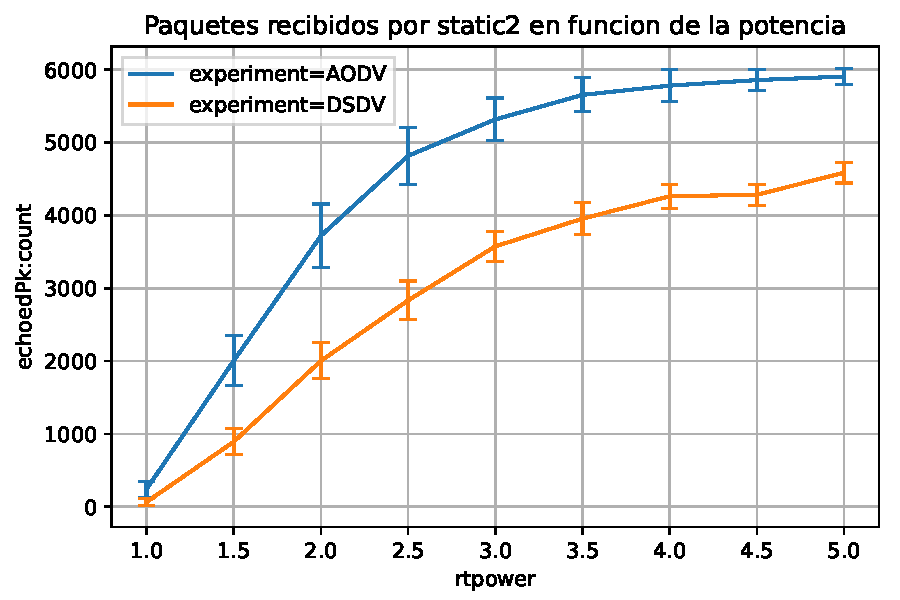
\includegraphics{imaxes/graficas/ejer4_1.pdf}
    \caption{Gráfica paquetes recibidos en static2 en función de la potencia}
    \label{fig:ejer4_1}
\end{figure}

\section{Ejercicio 4.2}

\subsection{Obtén una gráfica similar para el número de nodos. Explica lo observado.?}

\section{Ejercicio 4.3}

\subsection{Obtén una gráfica como las anteriores para la velocidad. Explica lo observado.}

\begin{figure}[H]
    \centering
    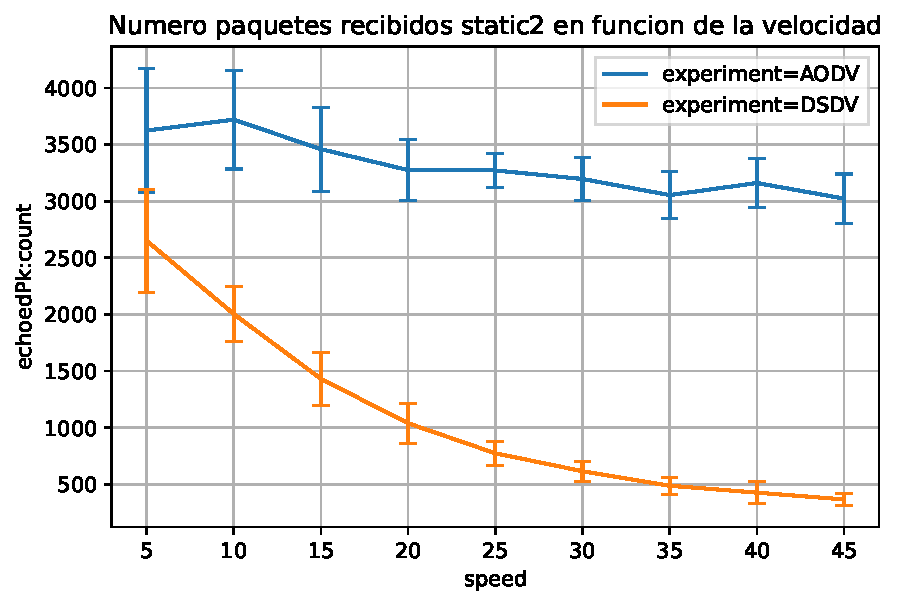
\includegraphics{imaxes/graficas/ejer4_3.pdf}
    \caption{Gráfica paquetes recibidos en static2 en función de la velocidad}
    \label{fig:ejer4_1}
\end{figure}

\section{Ejercicio 4.4}

\subsection{Para DSDV, obtén una gráfica del porcentaje de paquetes perdidos con diferentes valores de helloInterval.
Explica lo observado.}